\chapter{Costruzione di uno Spanning Tree}
%Tutti i protocolli visti fino ad ora, hanno un numero di messaggi pari a
%$\Omega(m)$, dato che si lavora su grafi generici. Al crescere della rete,
%aumentano gli archi e quindi aumentano il numero di messaggi nei nostri
%protocolli. Questo va contro corrente all'idea di ampliare la rete per
%velocizzare il nostro sistema. L'idea è quindi quella di costruire uno Spanning
%Tree (Albero di copertura) e sfruttarlo poi in tutte le istanze dei nostri
%protocolli.
In un ambiente distribuito, costruire uno Spanning Tree di un grafo $G$ significa
muovere il sistema da una configurazione iniziale dove ogni entità è solo a
conoscenza dei suoi vicini $N$, ad una configurazione dove:

\begin{enumerate}
    \item Ogni entità $x$ sceglie un sottoinsieme dei suoi vicini $N(x)$ come
          vicinato nello ST, chiamato $TREE\_NEIGHBORS(x)$;
    \item L'insieme dei link corrispondenti forma uno ST di $G$.
\end{enumerate}

Quello che si vuole quindi è un algoritmo che, una volta eseguito, garantisce la
costruzione di uno Spanning Tree $T(G)$ del grafo $G$.\\
\textbf{Le restrizioni} su cui faremo riferimento saranno $R+UI$.\\
Si noti che T non è noto a priori alle entità e potrebbe non esserlo dopo che è
stato costruito: un'entità deve solo sapere quali dei suoi vicini sono anche
suoi vicini nello spanning tree T.\\
%Formalmente: Quaderno
$P_{INIT} = $ Inizialmente nessun arco appartiene allo ST di un'entità $x$.\\
$P_{FINAL}$ = Per il suo calcolo si fanno riferimento ai tre punti successivi:
\begin{itemize}
    \item Per ogni entità, l'insieme degli archi che formano parte dell'albero
          sono comunque inclusi nei suoi vicini.
    \item Se un'entità sceglie un link, anche l'altra sarà obbligata a farlo
    \item Prese tutte le scelte dei collegamenti, esse formano un albero di
          copertura che è equivalente a quello originale.
\end{itemize}
In dettaglio:\\
$P_{INIT}$: $< \forall x \in \xi N_T(x) = \emptyset >$\\
$P_{FINAL}$: $< \forall x \in \xi N_T(x) \subset N(x) \land \cup_{x \in \xi}
    \equiv S.T.(G)>$

\section{Costruzione di uno Spanning tree con iniziatore unico: Protocollo
  \textit{Shout}} Le informazioni che un'entità possiede sono le etichette dei
numeri di porta dei suoi vicini e il fatto che, se si spedirà un messaggio,
allora prima o poi sarà sicuramente consegnato. Sotto queste affermazioni,
costruiamo un algoritmo per il calcolo dello ST attraverso i seguenti passi:

\begin{enumerate}
    \item L'iniziatore ``chiede'' al suo vicinato tramite un messaggio $Q$ di
          Broadcast "Sei un mio vicino nello ST?
    \item Un' entità $x \neq $ \texttt{initiator} che ha ricevuto $Q$, risponde
          ``\texttt{SI}'' solo se è la prima volta che riceve $Q$, ``\texttt{NO}''
          altrimenti. L'iniziatore risponde sempre ``\texttt{NO}''.
    \item Contestualmente all'invio di un ``\texttt{SI}'', un'entità manda $Q$ al
          suo vicinato tranne ai ``sender'' (ricordiamoci che stiamo utilizzando il
          Flooding).
    \item Ogni entità termina la propria esecuzione quando ha ricevuto una
          risposta da tutti i vicini a cui ha inviato $Q$.
\end{enumerate}
Per un' entità $x$ quindi, il suo vicinato nello ST sono i suoi vicini che hanno
risposto \texttt{SI}, mentre per l'iniziatore sono tutti i nodi ai quali è stato
inviato il messaggio $Q$.\\
Si ha quindi un \texttt{Broadcast} di $Q$ con una risposta per ogni $Q$ inviato.
Il protocollo Shout infatti può essere visto come:

\begin{center}
    \texttt{Shout} = \textbf{Flooding} + \textbf{Reply}
\end{center}

\begin{figure}[H]
    \centering
    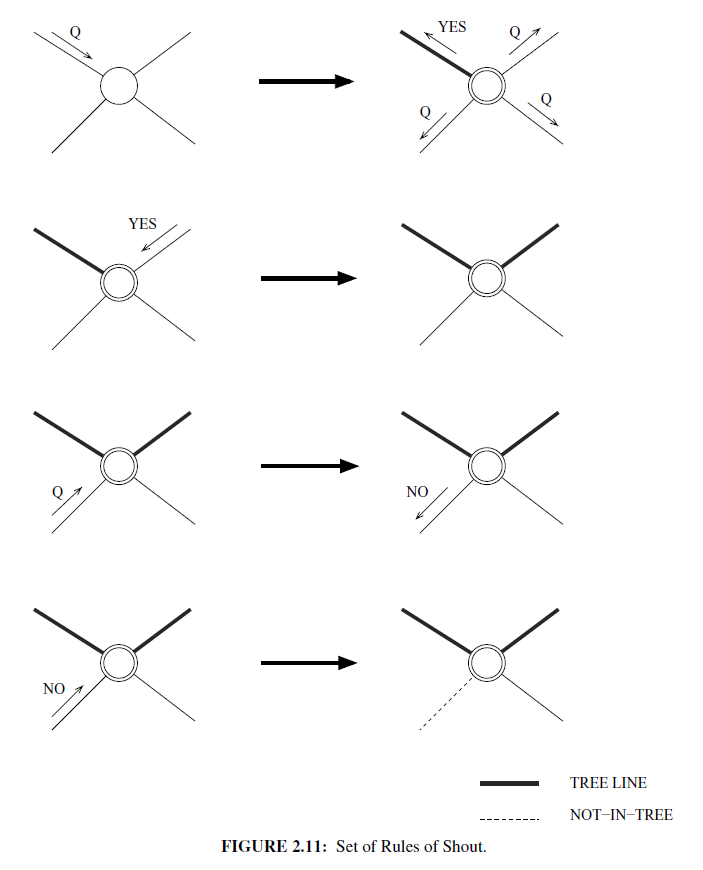
\includegraphics[width=15cm, keepaspectratio]{capitoli/costruzione-spanning-tree/imgs/dddd.png}
\end{figure}

\subsection{Correttezza del protocollo}
Dimostriamo ora che dopo l'esecuzione del protocollo Shout si ha sempre uno ST
radicato sul nodo iniziatore.

\begin{theorem}
    Il protocollo \texttt{Shout} termina correttamente.
\end{theorem}

\begin{proof}
    Questo protocollo consiste nel Flooding del messaggio $Q$. Data la
    correttezza del Flooding, è garantito che ogni nodo riceverà la domanda, e
    che quindi risponderà \texttt{SI} o \texttt{NO} ad ogni $Q$ che riceve. La terminazione segue
    proprio da questo. Per provare la sua correttezza bisogna dimostrare che il
    sotto grafo $G'$ definito dall'insieme $TREE\_NEIGHBORS$ è uno spanning tree
    di $G$, ossia è \textbf{Connesso}, \textbf{Contiene tutte le entità} e
    \textbf{Non contiene Cicli}. Osserviamo i seguenti tre punti:
    \begin{enumerate}
        \item \textbf{Connesso:} Se $x \in$ $T_N(y)$ allora $y \in$ $T_N(x)$
              (poiché all'invio di un ``\texttt{SI}'' un'entità accetta di
              essere figlia e l'altra apprende di essere padre).
        \item \textbf{Contiene tutte le entità:} Se un'entità $x$ invia un ``\texttt{SI}''
              ad $y$, allora $x \in T_N(y)$; inoltre è connessa all'iniziatore s
              da un cammino dove ``\texttt{SI}'' è stato inviato su ogni link.
              \begin{proof}[Dimostrazione. \textit{[Modo 1]}]
                  Supponiamo un nodo $x$ non raggiungibile dall'iniziatore $s$
                  dal grafo T indotto dalla relazione con il "padre". Questo
                  significa che $x$ non ha mai inviato un messaggio di \texttt{SI}, ma
                  questo implicherebbe che $x$ non ha mai ricevuto la domanda
                  $Q$. Ma questo è impossibile per la correttezza del flooding,
                  ogni entità ha per forza ricevuto il $Q$ e quindi $x$ non può
                  esistere.\\

                  In altre parole, se per assurdo
                  così non fosse, significherebbe che $x$ non ha mai inviato un
                  ``\texttt{SI}'' ma ciò è assurdo per la correttezza del
                  Flooding, poiché $x$ ha ricevuto sicuramente Q, e quindi ha
                  inviato un \texttt{SI}. Quindi l'albero ottenuto dopo
                  l'esecuzione sarà sicuramente connesso

                  \begin{center}
                      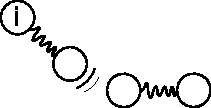
\includegraphics[scale=1]{capitoli/costruzione-spanning-tree/imgs/n_21}
                  \end{center}
              \end{proof}
        \item \textbf{Non contiene Cicli:} Ogni $x \neq $ \texttt{initiator}
              manda esattamente un solo messaggio ``\texttt{SI}''; se così non
              fosse, potrebbero essere presenti dei cicli che in un albero non
              possono essere presenti.
    \end{enumerate}
\end{proof}

Date queste supposizioni, il sottoinsieme $G'$ definito da tutti i
$TREE\_NEIGHBORS$ contiene tutte le entità, è connesso e non contiene cicli. È
possibile affermare che è uno Spanning Tree di $G$.\\
Si noti che $G'$ è in realtà un albero radicato nell'iniziatore. Ricordiamo che,
in un albero radicato, ogni nodo (tranne la radice) ha un genitore: il vicino
più vicino alla radice; tutti gli altri suoi vicini sono chiamati children. Il
vicino a cui $x$ invia un \texttt{SI} è il suo $genitore$; tutti i vicini da cui
riceve un \texttt{SI} sono suoi figli. Questo fatto può essere utile nelle operazioni
successive.\\
L'esecuzione del protocollo Shout termina con la terminazione locale: ogni
entità sa quando la propria esecuzione è terminata; questo si verifica quando
entra nello stato \textit{done}.\\
Si noti tuttavia che nessuna entità, incluso l'iniziatore, è a conoscenza della
terminazione globale (ovvero, ogni entità è terminata localmente). Questa
situazione è abbastanza comune nei calcoli distribuiti. Se è necessario che
l'iniziatore sappia che l'esecuzione è terminata (ad esempio, per avviare
un'altra attività), Flood + Reply può essere facilmente modificato per
raggiungere questo obiettivo.

\subsection{Costi}
Andiamo ora ad analizzare i costi del protocollo:

\underline{Messaggi:}
\begin{center}
    $M[$\texttt{Shout}$/RI] = 2 M[$\texttt{Flooding}$/RI] = 2(2m-n+1) = 4m - 2n +
        2 = O(m)$
\end{center}
\begin{center}
    $M[$\texttt{Shout}$/RI] = 4m - (2(n-1)) = O(m)$
\end{center}
Dove:
\begin{itemize}
    \item $4m$ sono i 4 messaggi per arco dati i ritardi di comunicazione
    \item Ai $4m$ messaggi sottraggo tutti gli archi in cui passa un $Q$ ed un
          \texttt{SI}, che sono appunto $(n-1) + (n-1)$.
\end{itemize}

Questo perché, se a seguito di una domanda rispondo ``\texttt{SI}'', sull'arco
passano 2 messaggi, ma se invio ``\texttt{NO}'', per i ritardi di comunicazione, posso
avere fino a quattro messaggi. Quindi ho 4 messaggi per arco, a cui sottraggo
però gli $2(n-1)$ archi su cui passano $(n-1)$ ``\texttt{SI}'' e $(n-1)$ $Q$.

\begin{figure}[H]
    \centering
    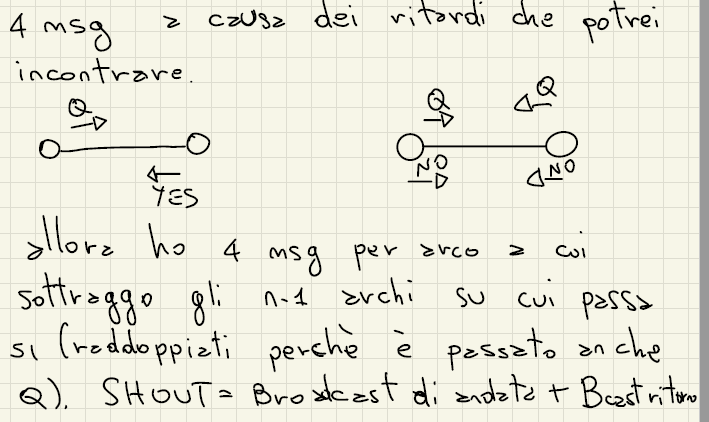
\includegraphics[width=\linewidth, keepaspectratio]{capitoli/costruzione-spanning-tree/imgs/hh}
\end{figure}

\underline{Tempo:}
\begin{center}
    $T[$\texttt{Shout}$/RI] = 1 + T[$\texttt{Flooding}$/RI] \leq d + 1 = O(d)$
\end{center}
Mandiamo i ``\texttt{SI}'' contemporaneamente ai $Q$; inoltre il $+1$ è per il
\texttt{NO} che risponderà l'ultimo nodo nel caso peggiore in cui avesse già
ricevuto la domanda Q da un'altra entità.

\begin{center}
    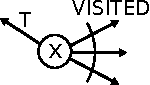
\includegraphics[scale=1]{capitoli/costruzione-spanning-tree/imgs/n_22}
\end{center}

\subsection{Protocollo Shout}
\begin{lstlisting} [caption={\textit{Protocollo Shout.}}]
S = {INITIATOR, ACTIVE, IDLE, DONE}
Restrictions = RI

INITIATOR 
    Spontaneously
    begin
        Tree-neighbors = $\emptyset$
        send(Q) to N(x)
        counter = 0
        become ACTIVE
    end

IDLE
    Receiving(Q)
    begin
        Tree-neighbors = {sender}
        send(YES) to sender
        counter = 1
        if counter = |N(x)| then
            become DONE
        else
            send(Q) to N(x)\sender
            become ACTIVE
    end

ACTIVE
    Receiving(Q)
    begin
        send(NO) to sender
    end
    
    Receiving(YES)
        begin
            Tree-neighbors =  Tree-neighbors $\cup$ {sender}
            counter = counter + 1
            if counter = |N(x)| then 
                become DONE        
        end
    
    Receiving(NO)
        begin
            counter = counter + 1
            if counter = |N(x)| then
            become DONE
        end
    
\end{lstlisting}

\subsection{Complessità del problema: Lower Bound}
Vediamo ora quanto ci costa, in generale, la costruzione di uno Spanning Tree:

\underline{Messaggi:}
\begin{center}
    $M[ST/RI] \geq m = \Omega(m)$
\end{center}

\begin{proof}
    Assumiamo che esista un protocollo $A$ corretto che, in ogni esecuzione
    sotto le restrizioni $R$ ed $UI$, in ogni Grafo utilizza un numero di
    messaggi $<m(G)$ per risolvere il problema della costruzione di uno spanning
    tree. Se cosi fosse ci sarebbe un arco in $G$ dove non transitano messaggi
    in nessuna direzione durante un esecuzione di $A$. Consideriamo l'esecuzione
    di $A$ in $G$ e sia $e=(x,y)$ l'arco dove non vengono trasmessi messaggi.
    Costruiamo ora un nuovo grafo $G'$ da $G$ ottenuto rimuovendo l'arco $e$ ed
    aggiungendo un nuovo nodo $z$ e due nuovi archi $e_1=(x,z)$ e $e_2=(y,z)$.
    Assumiamo che $z$ non sia iniziatore del protocollo. Eseguiamo ora la stessa
    identica esecuzione di $A$ nel nuovo grafo $G'$, dato che non transitavano
    messaggi tra $x$ ed $y$ è possibile eseguire la stessa esecuzione, poiché su
    $G'$ il link tra $x$ ed $y$ nemmeno è presente. Però dato che nessun
    messaggio transitava tra $x$ ed $y$, in $G'$ nessun messaggio transita tra
    $x$ e $z$ e $y$ e $z$, ma dato che $z$ non è iniziatore e non riceve nessun
    messaggio, non invierà mai una risposta. Questo significa che in tempo
    finito il protocollo $A$ termina, affermando che ha costruito una spanning
    tree di $G'$ ma in questo caso $z$ non è connesso all'albero costruito, quindi $A$
    non termina correttamente.
\end{proof}

\underline{Tempo:}
\begin{center}
    $T[$\texttt{ST}$/RI] \geq d(G) = \Omega(d)$
\end{center}
Per raggiungere il nodo più lontano abbiamo bisogno di $d$ step. Abbiamo quindi
che Shout è ottimo sia in termini di messaggi $\Theta(m)$, sia in termini di
tempo $\Theta(d)$.

\section{Shout+ miglioramento di Shout}
Possiamo ridurre il numero di messaggi inviati rimuovendo i messaggi di tipo
\texttt{NO}. Per ottenere questo possiamo fare in modo che la ricezione di un
messaggio di tipo $Q$ su un nodo che stà aspettando una risposta funzioni come
``\texttt{NO}'' implicito.\\
Prendiamo ad esempio un nodo $x$ che ha appena inviato un messaggio $Q$ al suo
vicino $y$.\\ Perché $y$ potrebbe rispondere \texttt{NO}? \\Risponderà così solo
se ha già ricevuto una domanda $Q$ e quindi già risposto \texttt{SI} a qualche
altra entità, in questo caso $y$ ha già inviato $Q$ allo stesso tempo a tutti
gli altri vicini, incluso $x$. Se $y$ risponde \texttt{NO} ad $x$, deve aver già
inviato $Q$ ad $x$. Possiamo ovviamente usare questa caratteristica a nostro
vantaggio, dopo che $x$ invia $Q$ ad $y$, se riceve \texttt{SI} sa che $y$ è un
suo vicino, se invece riceve $Q$, dedurrà che $y$ ha risposto \texttt{NO}.\\
In altre parole, quando un messaggio $Q$ arriva ad un nodo che sta aspettando una
risposta può essere inteso come una risposta negativa, quindi concludiamo che è
possibile non inviare messaggi di \texttt{NO}.
\begin{center}
    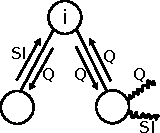
\includegraphics[scale=1.4]{capitoli/costruzione-spanning-tree/imgs/n_23}
\end{center}
\underline{Messaggi:}\\
Su ogni arco viaggiano quindi le coppie di messaggi ($Q$,\texttt{SI}) o
($Q$,$Q$)

\begin{center}
    $M[$\texttt{Shout+}$/RI] = 2m$ (è effettivamente =)\\
\end{center}

\underline{Tempo:}\\
Rispetto allo Shout risparmiano $1$, in quanto l'ultimo nodo non deve più
attendere un'unità di tempo per ricevere i \texttt{NO} (non ci sono).
\begin{center}
    $T[$\texttt{Shout+}$/RI] \leq d$
\end{center}

\section{Algoritmo Shout+ con più iniziatori}
Abbiamo assunto fino ad ora che tutti i protocolli avevano iniziatore unico, ma
come si comporterebbe il protocollo \texttt{Shout+} con più iniziatori?
\begin{center}
    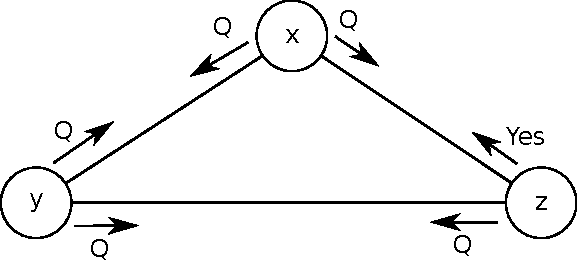
\includegraphics[scale=0.8]{capitoli/costruzione-spanning-tree/imgs/n_36}
\end{center}
Quando su un arco viaggiano due domande, l'arco \underline{non} appartiene allo
ST. \\
\texttt{Shout+} con più iniziatori \underline{non} funziona, perché \textbf{crea
    una foresta.}

\begin{theorem}
    Il problema dello ST è deterministicamente non risolvibile sotto R
    (togliendo l'UI), ovvero che non esiste un protocollo deterministico che
    termina sempre correttamente in un tempo finito.
\end{theorem}

\begin{proof}
    Per dimostrarlo prendiamo un grafo completo con 3 nodi ed etichettato come
    segue in figura.\\
    Supponiamo di avere un algoritmo deterministico $A$ e più iniziatori:
    \begin{center}
        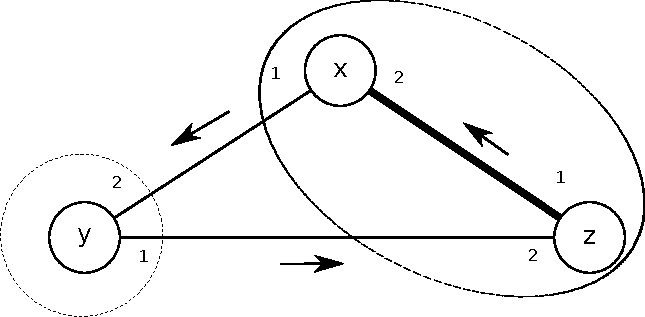
\includegraphics[scale=0.8]{capitoli/costruzione-spanning-tree/imgs/n_37}
    \end{center}

    Supponiamo che $x, y, z$ siano tutti e tre iniziatori, che siano nello
    stesso stato, che inizino contemporaneamente il protocollo e che abbiano
    tutti valori identici. Se $A$ è un protocollo che da soluzione al problema,
    dovrà funzionare sotto ogni condizioni di ritardo di messaggi e
    indipendentemente dal numero di iniziatori. Supponiamo di avere ritardo di
    comunicazione unitario, che sia presente la sincronia di Clock e che tutte
    le entità inizino contemporaneamente l'esecuzione del protocollo $A$. Dato
    che sono in stati identici (stessi valori iniziali e stessi numeri di
    porta), le entità eseguiranno le stesse computazioni, ottenendo gli stessi
    risultati (continuando ad avere gli stessi valori locali), inviare gli
    stessi messaggi agli stessi numeri di porta ed entrare eventualmente nel
    nuovo stato tutte insieme. In pratica tutte le entità continueranno ad
    essere completamente identiche. Se $A$ da soluzione al protocollo, deve
    terminare in tempo finito. Nel nostro caso $A$ dovrà solamente eliminare un
    arco per far si che si ottenga uno Spanning Tree; prendiamo per esempio
    l'arco $(x,y)$. In questo caso la variabile $TREE\_NEIGHBORS$ sarà la porta
    con la label 2 dell'entità $x$ e la porta 1 dell'entità $y$, invece $z$ ha come
    $TREE\_NEIGHBORS$ porta \{1, 2\}. In altri termini, quando il protocollo
    termina, tutte le entità hanno differenti valori per la variabile locale
    $TREE\_NEIGHBORS$ ma questo è impossibile poiché per supposizione gli stati
    delle entità devono essere necessariamente identici.

    %Siccome $x, y, z$ hanno la stessa esecuzione e partono dallo stesso stato,
    %in ogni momento, calcoleranno sempre lo stesso risultato e saranno quindi
    %sempre nello stesso stato; quindi alla fine abbiamo o che tutti gli archi
    %appartengono a ST, o nessuno. Ciò è \textbf{assurdo}.

\end{proof}

\begin{center}
    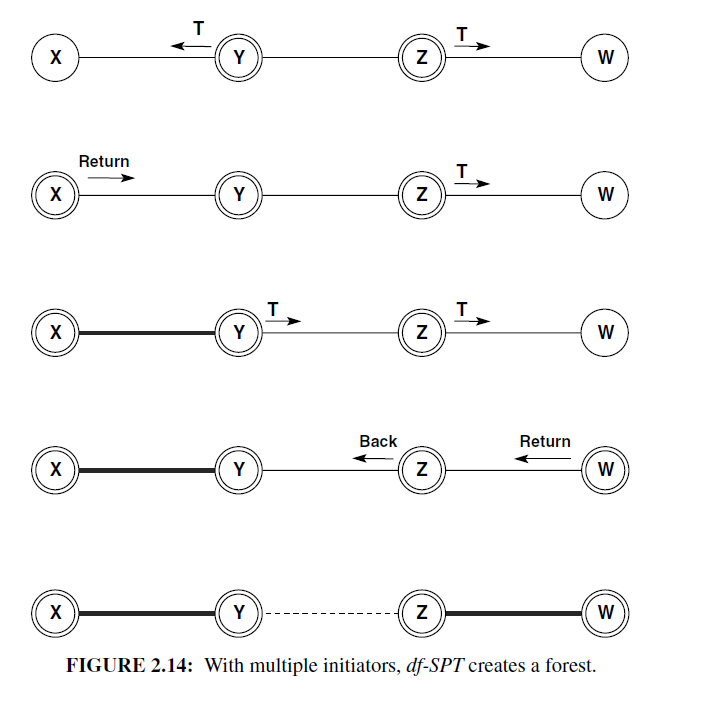
\includegraphics[scale=0.6]{capitoli/attraversamento/imgs/asd.png}
\end{center}

\textbf{Causa del fallimento}\\
La causa per cui il protocollo \texttt{Shout} con più iniziatori fallisce è che
un'entità non riesce a distinguere tra le varie richieste che gli vengono
inviate. Quindi il più semplice approccio sarebbe quello di aggiungere un id ad
ogni messaggio di ``$Q$'' e ``\texttt{SI}'' così da identificarle.

Dobbiamo trovare l'insieme di restrizioni "minimo" (oltre a $R$) che ci permetta
di costruire correttamente lo ST con più iniziatori.

\section{Spanning Tree con valori iniziali delle entità distinti}
Possiamo risolvere il problema aggiungendo una singola restrizione all'insieme
$R$: ogni entità ha un valore iniziale unico (id) che permette di distinguerla
dalle altre. Quando un'entità invia un messaggio invia anche l'id dell'
iniziatore.

\begin{center}
    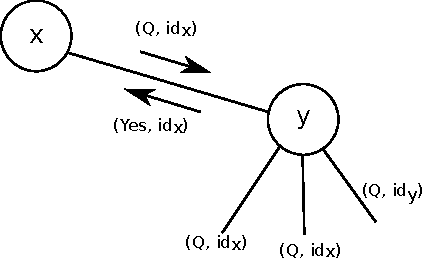
\includegraphics[scale=0.8]{capitoli/costruzione-spanning-tree/imgs/n_38}
\end{center}

L'applicazione di questo approccio risulta nell'avere ogni iniziatore che
costruisce il proprio spanning tree radicato in lui e che utilizza l'id degli
altri iniziatori per distinguere tra le diverse costruzioni. Quindi invece che
cooperare per la costruzione di un singolo spanning tree, si avranno
contemporaneamente più spanning tree indipendentemente costruiti. Questo implica
che  tutti i messaggi del protocollo (Ovvero messaggi di ``$Q$'' e messaggi di
``\texttt{SI}'' nel protocollo \texttt{Shout+}) abbiano l'id dell'iniziatore. Sono
richieste inoltre variabili addizionali poiché in ogni entità saranno presenti
più istanze della variabile $TREE\_NEIGHBORS$, ovvero uno per ogni spanning tree
che sta venendo costruito. Inoltre, ogni entità sarà in un differente stato per
ognuna di queste costruzioni. Ricordiamoci che il numero di iniziatori non è
noto a priori e può cambiare ad ogni esecuzione. In questo modo costruiamo $K^*$
ST con $K^*=$ numero di iniziatori. Siccome \texttt{Shout+} ci costa $2m$, il
costo è:

$$2m K^* = O(n^3)$$

poiché $1 \leq K^* \leq n$. %e poiché si sta costruendo non uno ma ma K* ST.

Ogni nodo può distinguere a quanti ST sta partecipando in base all'id dei
messaggi.

\subsection{Algoritmo MultiShout}
Consideriamo adesso un algoritmo basato sul protocollo \textbf{Shout+} con un
metodo migliore: Un approccio migliore è quello di lasciare ad ogni iniziatore
la possibilità di costruire il suo ST, ma di scegliere di far sopravvivere
localmente solamente la costruzione con id \underline{minimo}. Quando un'entità
si interfaccia con differenti costruzioni di uno ST, sceglierà sempre quella con
id minore e terminerà quelle che conosce. I vantaggi di questo approccio sono:

\begin{enumerate}
    \item Ogni entità è coinvolta in una singola costruzione di uno ST.
    \item In terminazione, tutte le entità avranno un singolo ST in comune.
\end{enumerate}

Gli stati di questo protocollo sono IDLE, ACTIVE e DONE. Tutte le entità
iniziano in stato di IDLE ed in terminazione tutte le entità saranno in stato di
DONE.

Riassumendo quindi, quando un nodo $x$ che sta portando avanti la costruzione di
un albero radicato in $z$ con $id_z$ (il nodo $z$ può essere anche $x$ stesso)
riceve un messaggio con $id_y$ tale che:

$$
    id_y < id_z
$$

Allora $x$ smette di lavorare per l'entità a cui stava portando avanti la
costruzione dello spanning tree e porta avanti la costruzione dello spanning
tree radicato in $y$. Il punto fondamentale di questo approccio è che solo lo ST
con id minimo viene portato a termine tra gli iniziatori, quindi
\texttt{MultiShout} costruisce un albero radicato sull'iniziatore con id minimo.
Di conseguenza, i nodi conservano solo i dati relativi ad un singolo ST.\\
Per come si è costruito il protocollo però, quando un'entità ha concluso la sua
costruzione, non sa se dovrà iniziare a lavorare nuovamente per qualcun altro,
in quanto è possibile che un'entità che abbia terminato riceva un messaggio da
un altro iniziatore (con la possibilità di avere id minore). Quindi è necessario
includere nel protocollo un meccanismo che permetta la terminazione locale delle
entità. \\
\textit{Problema del protocollo:} \textbf{i nodi non hanno conoscenza locale di
    terminazione:} una possibile soluzione è fare in modo che le foglie dell'unico
ST che viene portato a termine mandino al proprio padre un messaggio di fine
lavoro fino alla radice, la quale diventa cosciente della fine del suo lavoro ed
invia un messaggio di terminazione in broadcast. Possiamo vedere questo
passaggio come un:

$$
    \textit{Convergecast + Broadcast}
$$

\begin{theorem}
    Il protocollo MultiShout costruisce un ST radicato nell'iniziatore con
    id più piccolo tra gli iniziatori.
\end{theorem}

\begin{proof}
    Sia $s$ l'inizializzatore con id minore, consideriamo un altro iniziatore $x$
    diverso da $s$. Da $x$ verrà costruito quindi lo spanning tree radicato in lui,
    che chiameremo $T_x$. Dimostriamo due punti fondamentali:
    \begin{enumerate}
        \item \textbf{La costruzione di $T_x$ non verrà completata:} Osserviamo
              che $T_x$ deve contenere tutti i nodi, incluso $s$, ma quando $s$
              riceve un messaggio relativo alla costruzione di un altro ST,
              avendo id minore di tutti, ignorerà il messaggio uccidendo la
              costruzione di quell'albero.
        \item \textbf{La costruzione di $T_s$ verrà completata:} Dato che l'id
              di $s$ è il minore di tutti, nessuna entità ignorerà il messaggio
              e quindi lo ST sarà completato.
    \end{enumerate}
\end{proof}

\subsubsection{Complessità}
Supponiamo di avere $K^*$ iniziatori connessi ognuno con un solo nodo nel sotto
grafo $k_{n-K^*}$ completamente connesso (completo).
\begin{center}
    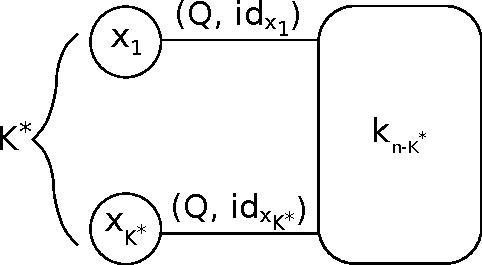
\includegraphics[scale=0.9]{capitoli/costruzione-spanning-tree/imgs/n_39}
\end{center}
Inoltre, con $id_{x_1} > id_{x_2} > \cdots > id_{x_{K^*}}$.

Supponiamo adesso un'esecuzione dove i messaggi $Q$ che inviano i $K^*$ iniziatori
arrivano sul grafo completo in un ordine in base al loro indice, quindi $x_1$
arriva per primo, poi $x_2$ arriva per secondo e così via. Quando il messaggio
$Q$ di $x_1$ arriva negli $n-K^*$ nodi, si genererà la costruzione dello
spanning tree radicato in lui. Assumiamo adesso che prima che il messaggio $Q$
di $x_2$ arrivi nel grafo completamente connesso, la computazione di $x_1$
dentro il suddetto grafo sia conclusa, pagando quindi $O(n-k^*)^2$. Quando $Q$
di $x_2$ arriva nel grafo completamente connesso, tutto il lavoro
precedentemente svolto da $x_1$ è da buttare via, poiché tutti i nodi adesso
devono seguire la sua costruzione dello ST, avendo id più piccolo di $x_1$. Se
si continuasse in questo modo, $O(n-k^*)^2$ verrebbe ripetuto per $K^*$ volte,
per un totale di:

%Supponiamo ora che $x_1$ parta per primo e che inizi a costruire uno ST in
%$k_{n-K^*}$ pagando $2m = O(n^2)$. Assumiamo adesso che la costruzione dello ST
%radicato in $x_1$ sia conclusa (pagando quindi $O(n-k^*)^2$) prima che il
%messaggio Q di $x_2$ venga spedito all'interno del suddetto grafo. Tutto il
%lavoro fatto da $x_1$ è da buttare, poiché adesso i nodi dovranno seguire la
%costruzione dello spanning tree radicato in $x_2$. Si va avanti così fino a
%$x_{K^*}$, disfacendo di volta in volta il lavoro precedente.

\underline{Messaggi:}
\begin{center}
    $M[$\texttt{MultiShout}$] = O(k^*(n-k^*)^2)) + (n-1)+ (n-1) = O(n^3)$\\
    con $k$ frazione lineare rispetto ad $n$, ad esempio $k=\frac{n}{2}$
\end{center}
$k^*$ volte invio un messaggio in un grafo completo (archi = $m^2$) dato che
$m=n-k^*$. E $(n-1)$, $(n-1)$ è per Convergecast e Broadcast in un albero (un
messaggio per nodo).

\underline{Tempo:}
\begin{center}
    $T[$\texttt{MultiShout}$] \leq d + 1 + 2d = 3d + 1$
\end{center}
Dove:
\begin{itemize}
    \item  $d+1$ è il tempo speso per la costruzione dello ST attraverso il
          protocollo Shout
    \item $2d$ è il costo del Broadcast e Convergecast che parte dal minimo
          necessario per la terminazione del protocollo
\end{itemize}
%il $2d$ è per il tempo speso per effettuare il convergecast e broadcast del
%minimo finale, mentre lo $d+1$ è il tempo speso da normale protocollo di shout
%per la creazione dello ST.

\section{ST con altri protocolli e Iniziatore Unico}
Possiamo costruire uno Spanning Tree usando protocolli che risolvono il problema
del Broadcast o dell'Attraversamento, opportunamente modificati.

\subsection{ST con Traversal normale DF}
Sappiamo che l'applicazione del protocollo \texttt{DF} costruisce già effettivamente
uno Spanning Tree del grafo che stiamo considerando. Questo è ottenuto
rimuovendo gli archi dove transita un messaggio di BACKEDGE da $G$. In altre
parole, l'insieme $TREE\_NEIGHOBRS$ di un'entità $x$ saranno tutte le entità dalle
quali riceverà un messaggio di RETURN, e se $x$ non è l'iniziatore, l' entità
dalla quale $x$ ha ricevuto $T$ per la prima volta.

\subsection{ST con Traversal normale DF*}
Il protocollo utilizza una visita in \textit{profondità}, quindi se ad esempio
lo facessimo girare su un grafo completo (quindi $d(G)=1$) mi darebbe un output
uno Spanning Tree dove $d(T) = n-1$. Visto che il nostro scopo è quello di
costruire un albero di copertura per far girare i protocolli visti, e questi
hanno complessità temporale che dipende dal diametro della rete, impiegherebbero
un tempo elevato per il raggiungimento dell'obiettivo. Il nostro scopo è quello
di avere $d(T) \leq 2d(G)$. Infine, il numero di messaggi da utilizzare per la
costruzione dell'albero risulta essere troppo alto per i nostri scopi (circa
$4m$).

\subsection{ST con Broadcasting}

\begin{theorem}
    L'esecuzione di qualsiasi protocollo di Broadcasting può essere modificata
    per costruire uno Spanning Tree.
\end{theorem}

Prendiamo un qualsiasi protocollo di broadcasting $B$. Da come abbiamo definito il
broadcast, tutte le entità riceveranno l'informazione $I$ che inizialmente ha
solo l'iniziatore.
Visto che i protocolli che utilizzano la DFS ci costruivano alberi ``alti'',
proviamo ad utilizzare la visita in \textit{ampiezza}.

\subsubsection{BFS}
Per la costruzione dello Spanning Tree tramite la BFS, utilizziamo la seguente
strategia.
\textbf{Strategia:}
\begin{enumerate}
    \item determinare il nodo con eccentricità minore (quello che detta
          l'eccentricità di $G$, ossia il \textit{nodo centrale});
    \item costruire un BF-ST radicato su tale nodo.
\end{enumerate}

\begin{center}
    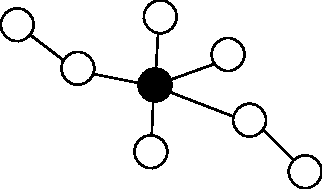
\includegraphics[scale=1]{capitoli/costruzione-spanning-tree/imgs/n_24}
\end{center}

\subsubsection{Eccentricità}
L'eccentricità di un qualunque nodo $x$ è definita come:
$$
    r_G(x) = \max\{\delta_G(x,y), y \in V(G)\}
$$
Quella di un grafo invece:
$$
    r(G) = \min \{ r_G(x), x \in V \}
$$

Il nodo \emph{x} con eccentricità minima in $G$ è detto \textbf{centro di $G$}
(in un grafo completo sono tutti centri).\\

Se si fa una BFS partendo da un centro (possono essere molteplici) otteniamo lo
ST più basso possibile. Infatti tale albero avrà altezza $r(G)$, possiamo quindi
dire che: $2 d_G \geq d_{BFS} \geq d_G$.
%Ove $d_G$ è il diametro del grafo [\ref{def_diametro}].

Per costruire uno ST con BFS, sotto restrizioni di iniziatore unico si può fare
nel seguente modo:

\begin{enumerate}
    \item Iniziatore manda un messaggio in broadcast ai vicini e attende la risposta
    \item Quando l'iniziatore ha avuto tutte le risposte rinvia un messaggio (tipo
          TOKEN)
    \item L'entità che lo riceve fa partire la costruzione nel nuovo livello
          come visto sopra e poi rinvia il TOKEN all'iniziatore che lo invierà
          al fratello.
\end{enumerate}

Il costo è $\mathcal{O}(n^2)$, considerando i seguenti tipi di messaggio:
\begin{itemize}
    \item $Q = 2m - n +1$
    \item $\text{\texttt{SI}, \texttt{NO}} = 2m -n +1$
    \item $T = 2n r(g)$
\end{itemize}
